% figs.tex -- renders the four manuscript figures as a tightly-cropped,
% multi-page PDF (one figure per page) for inclusion in main.tex via
% \includegraphics[page=N]{figs}. Compile: tectonic figs.tex  (or pdflatex).
\documentclass[crop,multi=tikzpicture,border=4pt]{standalone}
\usepackage{amsmath,amssymb}
\usepackage{xcolor}
\usepackage{tikz}
\usepackage{pgfplots}
\pgfplotsset{compat=1.17}
\usetikzlibrary{arrows.meta,positioning,fit,backgrounds,calc,shapes.geometric}

\definecolor{qpurple}{RGB}{106,61,154}
\definecolor{qblue}{RGB}{31,119,180}
\definecolor{qgreen}{RGB}{44,140,80}
\definecolor{qorange}{RGB}{214,118,32}
\definecolor{qgray}{RGB}{90,90,90}
\definecolor{lightq}{RGB}{233,226,245}
\definecolor{lightc}{RGB}{223,238,247}
\newcommand{\tpr}{\mathrm{TPR}}
\newcommand{\fpr}{\mathrm{FPR}}

\begin{document}

% ===== Page 1: Figure 1 -- hybrid architecture =====
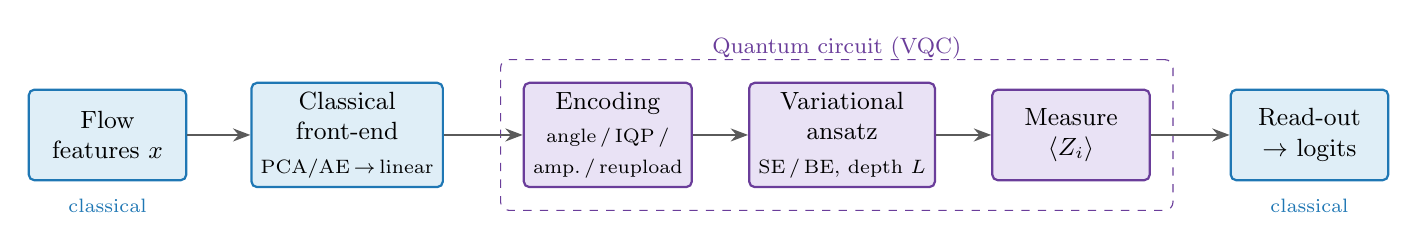
\begin{tikzpicture}[
  font=\small,
  box/.style={rounded corners=2pt,draw,minimum height=1.15cm,minimum width=2.0cm,align=center,thick},
  cbox/.style={box,fill=lightc,draw=qblue},
  qbox/.style={box,fill=lightq,draw=qpurple},
  arr/.style={-{Stealth[length=2.2mm]},thick,qgray},
  ]
  \node[cbox] (in) {Flow\\features $x$};
  \node[cbox,right=0.8cm of in] (pre) {Classical\\front-end\\[1pt]\scriptsize PCA/AE\,$\to$\,linear};
  \node[qbox,right=1.0cm of pre] (enc) {Encoding\\[1pt]\scriptsize angle\,/\,IQP\,/\\\scriptsize amp.\,/\,reupload};
  \node[qbox,right=0.7cm of enc] (ans) {Variational\\ansatz\\[1pt]\scriptsize SE\,/\,BE, depth $L$};
  \node[qbox,right=0.7cm of ans] (meas) {Measure\\$\langle Z_i\rangle$};
  \node[cbox,right=1.0cm of meas] (out) {Read-out\\$\to$ logits};
  \draw[arr] (in)--(pre); \draw[arr] (pre)--(enc); \draw[arr] (enc)--(ans);
  \draw[arr] (ans)--(meas); \draw[arr] (meas)--(out);
  \begin{scope}[on background layer]
    \node[draw=qpurple,dashed,rounded corners=3pt,fit=(enc)(ans)(meas),
          inner sep=8pt] (qbox-fit) {};
  \end{scope}
  \node[qpurple,font=\footnotesize] at ([yshift=4pt]qbox-fit.north) {Quantum circuit (VQC)};
  \node[below=0.1cm of in,qblue,font=\scriptsize] {classical};
  \node[below=0.1cm of out,qblue,font=\scriptsize] {classical};
\end{tikzpicture}

% ===== Page 2: Figure 2 -- attribution audit =====
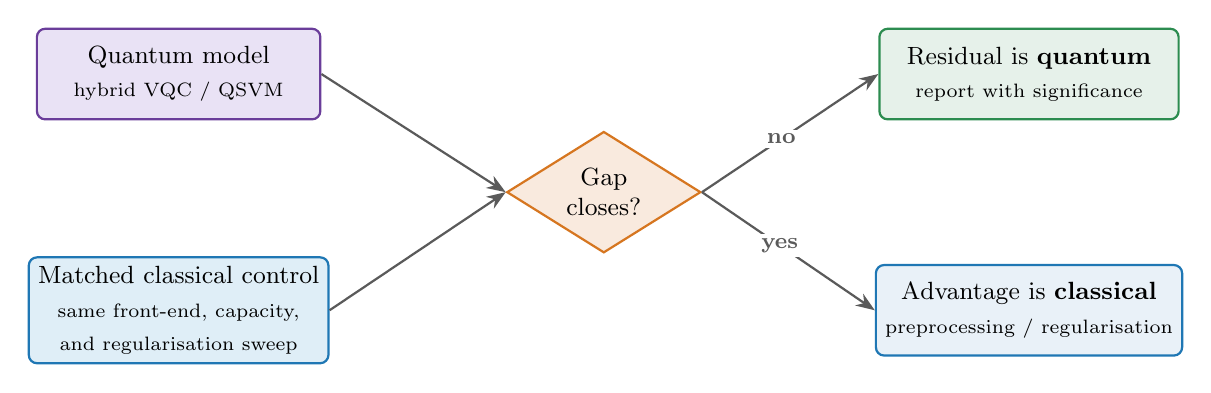
\begin{tikzpicture}[
  font=\small,
  qb/.style={rounded corners=3pt,draw=qpurple,fill=lightq,thick,minimum width=3.6cm,minimum height=1.15cm,align=center},
  cb/.style={rounded corners=3pt,draw=qblue,fill=lightc,thick,minimum width=3.6cm,minimum height=1.15cm,align=center},
  res/.style={rounded corners=3pt,draw=qgreen,fill=qgreen!12,thick,minimum width=3.8cm,minimum height=1.15cm,align=center},
  cl/.style={rounded corners=3pt,draw=qblue,fill=qblue!10,thick,minimum width=3.8cm,minimum height=1.15cm,align=center},
  dec/.style={diamond,aspect=1.6,draw=qorange,thick,fill=qorange!15,align=center,inner sep=3pt,minimum width=2.0cm},
  arr/.style={-{Stealth[length=2.4mm]},thick,qgray},
  lbl/.style={font=\footnotesize\bfseries,fill=white,inner sep=1.5pt},
  ]
  \node[qb] (q)  at (0, 1.5)  {Quantum model\\[1pt]\scriptsize hybrid VQC / QSVM};
  \node[cb] (c)  at (0,-1.5)  {Matched classical control\\[1pt]\scriptsize same front-end, capacity,\\[1pt]\scriptsize and regularisation sweep};
  \node[dec] (d) at (5.4, 0)  {Gap\\closes?};
  \node[res] (qu)  at (10.8, 1.5)  {Residual is \textbf{quantum}\\[1pt]\scriptsize report with significance};
  \node[cl]  (cla) at (10.8,-1.5)  {Advantage is \textbf{classical}\\[1pt]\scriptsize preprocessing / regularisation};
  \draw[arr] (q.east)   -- (d.west);
  \draw[arr] (c.east)   -- (d.west);
  \draw[arr] (d.east)   -- node[lbl,pos=0.45]{no}  (qu.west);
  \draw[arr] (d.east)   -- node[lbl,pos=0.45]{yes} (cla.west);
\end{tikzpicture}

% ===== Page 3: Figure 3 -- classical vs quantum F1 bars =====
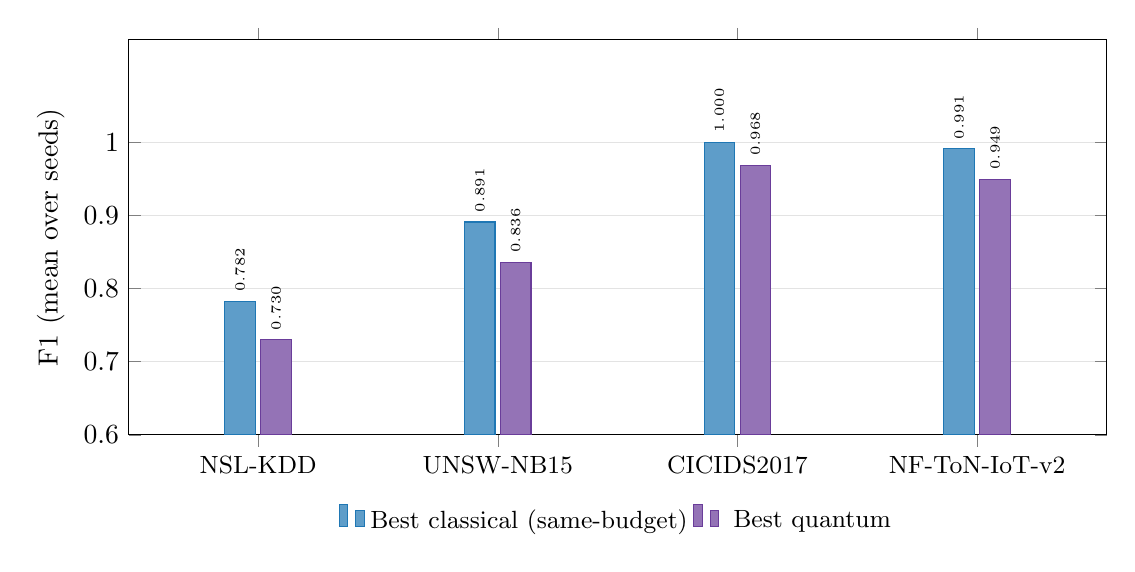
\begin{tikzpicture}
\begin{axis}[
  ybar, bar width=11pt,
  width=14cm, height=6.6cm,
  enlarge x limits=0.18,
  ymin=0.6, ymax=1.14,
  ytick={0.6,0.7,0.8,0.9,1.0},
  ylabel={F1 (mean over seeds)},
  symbolic x coords={NSL-KDD,UNSW-NB15,CICIDS2017,NF-ToN-IoT-v2},
  xtick=data,
  x tick label style={font=\small},
  legend style={at={(0.5,-0.16)},anchor=north,legend columns=2,font=\small,draw=none},
  nodes near coords,
  every node near coord/.append style={font=\tiny,rotate=90,anchor=west,
    /pgf/number format/.cd,fixed,fixed zerofill,precision=3},
  ymajorgrids,grid style={gray!22},
]
\addplot[fill=qblue!72,draw=qblue] coordinates
  {(NSL-KDD,0.782)(UNSW-NB15,0.891)(CICIDS2017,1.000)(NF-ToN-IoT-v2,0.991)};
\addplot[fill=qpurple!72,draw=qpurple] coordinates
  {(NSL-KDD,0.730)(UNSW-NB15,0.836)(CICIDS2017,0.968)(NF-ToN-IoT-v2,0.949)};
\legend{Best classical (same-budget),\ Best quantum}
\end{axis}
\end{tikzpicture}

% ===== Page 4: Figure 4 -- qubit-count ablation =====
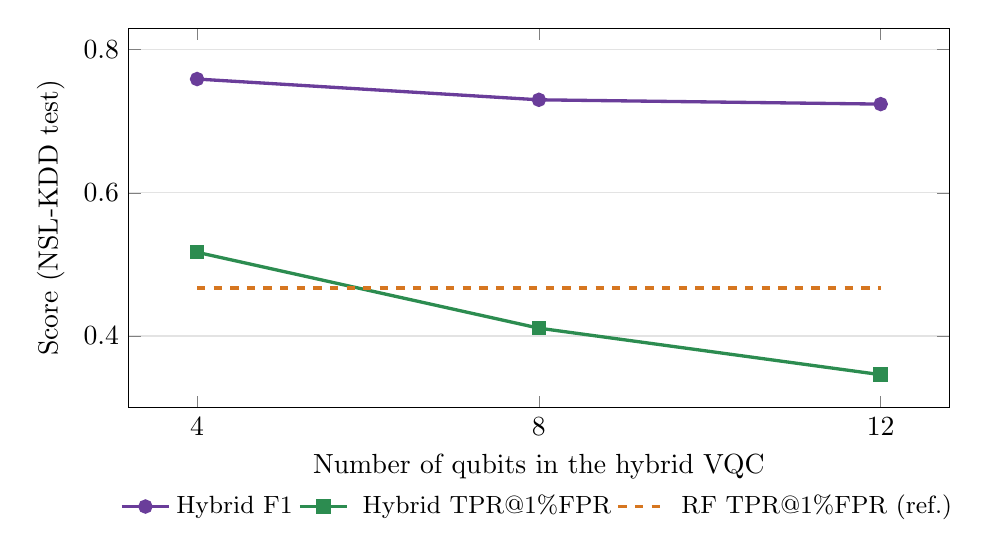
\begin{tikzpicture}
\begin{axis}[
  width=12cm, height=6.4cm,
  xlabel={Number of qubits in the hybrid VQC},
  ylabel={Score (NSL-KDD test)},
  xtick={4,8,12}, ymin=0.30, ymax=0.83,
  legend style={at={(0.5,-0.20)},anchor=north,legend columns=3,font=\small,draw=none},
  ymajorgrids,grid style={gray!22},
  every axis plot/.append style={very thick},
]
\addplot[qpurple,mark=*] coordinates {(4,0.759)(8,0.730)(12,0.724)};
\addplot[qgreen,mark=square*] coordinates {(4,0.517)(8,0.411)(12,0.346)};
\addplot[qorange,dashed,mark=none] coordinates {(4,0.467)(12,0.467)};
\legend{Hybrid F1,\ Hybrid $\tpr$@$1\%\fpr$,\ RF $\tpr$@$1\%\fpr$ (ref.)}
\end{axis}
\end{tikzpicture}

\end{document}
